\chapter{Árboles de expansión}

\index{{\'a}rbol!de expansión}
\indexaltsub{{\'a}rbol}{recubridor}
\indexaltsub{{\'a}rbol}{generador}

Un \key{árbol de expansión}, \textit{recubridor}, o \textit{generador}
de un grafo consiste en todos los nodos del grafo y algunas de sus
aristas, tal que haya un camino entre cualquier par de nodos.
Como los árboles en general, los árboles de expansión son
conexos y acíclicos. Usualmente hay múltiples maneras de
construir un árbol de expansión.

Por ejemplo, considera el siguiente grafo:
\begin{center}
    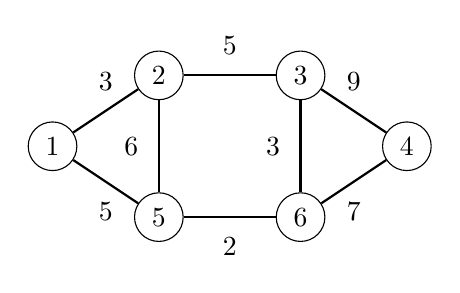
\begin{tikzpicture}[scale=0.9]
        \node[draw, circle] (1) at (1.5,2) {$1$};
        \node[draw, circle] (2) at (3,3) {$2$};
        \node[draw, circle] (3) at (5,3) {$3$};
        \node[draw, circle] (4) at (6.5,2) {$4$};
        \node[draw, circle] (5) at (3,1) {$5$};
        \node[draw, circle] (6) at (5,1) {$6$};
        \path[draw,thick,-] (1) -- node[font=\small,label=above:3] {} (2);
        \path[draw,thick,-] (2) -- node[font=\small,label=above:5] {} (3);
        \path[draw,thick,-] (3) -- node[font=\small,label=above:9] {} (4);
        \path[draw,thick,-] (1) -- node[font=\small,label=below:5] {} (5);
        \path[draw,thick,-] (5) -- node[font=\small,label=below:2] {} (6);
        \path[draw,thick,-] (6) -- node[font=\small,label=below:7] {} (4);
        \path[draw,thick,-] (2) -- node[font=\small,label=left:6] {} (5);
        \path[draw,thick,-] (3) -- node[font=\small,label=left:3] {} (6);
    \end{tikzpicture}
\end{center}

Un árbol de expansión para el grafo es el siguiente:
\begin{center}
    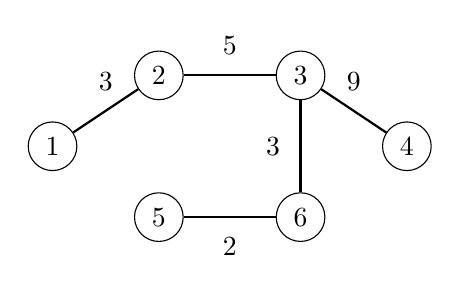
\begin{tikzpicture}[scale=0.9]
        \node[draw, circle] (1) at (1.5,2) {$1$};
        \node[draw, circle] (2) at (3,3) {$2$};
        \node[draw, circle] (3) at (5,3) {$3$};
        \node[draw, circle] (4) at (6.5,2) {$4$};
        \node[draw, circle] (5) at (3,1) {$5$};
        \node[draw, circle] (6) at (5,1) {$6$};
        \path[draw,thick,-] (1) -- node[font=\small,label=above:3] {} (2);
        \path[draw,thick,-] (2) -- node[font=\small,label=above:5] {} (3);
        \path[draw,thick,-] (3) -- node[font=\small,label=above:9] {} (4);
        \path[draw,thick,-] (5) -- node[font=\small,label=below:2] {} (6);
        \path[draw,thick,-] (3) -- node[font=\small,label=left:3] {} (6);
    \end{tikzpicture}
\end{center}

El peso de un árbol de expansión es la suma de los pesos de todas
sus aristas. Por ejemplo, el peso del árbol de expansión anterior es
$3+5+9+3+2=22$.

\index{{\'a}rbol!de expansión!mínimo}

Un \key{árbol de expansión mínimo} (MST, por \textit{minimum spanning tree})
es un árbol de expansión cuyo peso es tan pequeño como sea posible.
El peso de un árbol de expansión mínimo para el grafo de ejemplo es
20, y puede construirse de la siguiente manera:
\begin{center}
    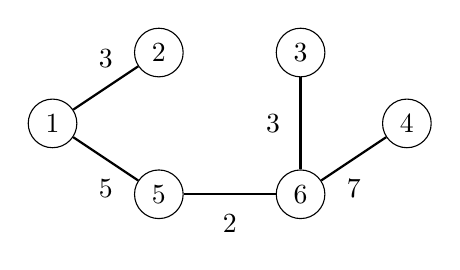
\begin{tikzpicture}[scale=0.9]
        \node[draw, circle] (1) at (1.5,2) {$1$};
        \node[draw, circle] (2) at (3,3) {$2$};
        \node[draw, circle] (3) at (5,3) {$3$};
        \node[draw, circle] (4) at (6.5,2) {$4$};
        \node[draw, circle] (5) at (3,1) {$5$};
        \node[draw, circle] (6) at (5,1) {$6$};

        \path[draw,thick,-] (1) -- node[font=\small,label=above:3] {} (2);
        \path[draw,thick,-] (1) -- node[font=\small,label=below:5] {} (5);
        \path[draw,thick,-] (5) -- node[font=\small,label=below:2] {} (6);
        \path[draw,thick,-] (6) -- node[font=\small,label=below:7] {} (4);
        \path[draw,thick,-] (3) -- node[font=\small,label=left:3] {} (6);
    \end{tikzpicture}
\end{center}

\index{{\'a}rbol!de expansión!máximo}

Similarmente, un \key{árbol de expansión máximo} es un árbol de expansión
cuyo peso es tan grande como sea posible. El peso de un árbol de expansión
máximo para el grafo de ejemplo es 32:
\begin{center}
    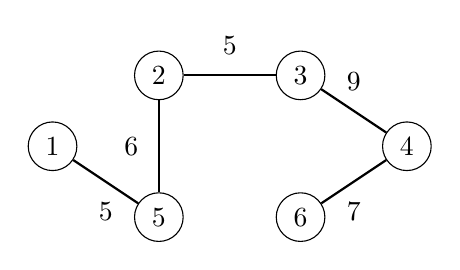
\begin{tikzpicture}[scale=0.9]
        \node[draw, circle] (1) at (1.5,2) {$1$};
        \node[draw, circle] (2) at (3,3) {$2$};
        \node[draw, circle] (3) at (5,3) {$3$};
        \node[draw, circle] (4) at (6.5,2) {$4$};
        \node[draw, circle] (5) at (3,1) {$5$};
        \node[draw, circle] (6) at (5,1) {$6$};
        \path[draw,thick,-] (2) -- node[font=\small,label=above:5] {} (3);
        \path[draw,thick,-] (3) -- node[font=\small,label=above:9] {} (4);
        \path[draw,thick,-] (1) -- node[font=\small,label=below:5] {} (5);
        \path[draw,thick,-] (6) -- node[font=\small,label=below:7] {} (4);
        \path[draw,thick,-] (2) -- node[font=\small,label=left:6] {} (5);
    \end{tikzpicture}
\end{center}

Ten en cuenta que un grafo puede tener varios árboles de expansión
máximos y mínimos, así que los árboles no son únicos.

Resulta que existen varios métodos voraces para construir árboles
de expansión mínimos y máximos. En este capítulo, veremos dos algoritmos
que procesan las aristas de un grafo ordenadas por sus pesos.
Nos concentraremos en encontrar árboles mínimos, pero los mismos
algoritmos aplican para encontrar árboles máximos si procesamos
las aristas en orden inverso.

\section{Algoritmo de Kruskal}

\index{algoritmo de!Kruskal}

En el \key{algoritmo de Kruskal},\footnote{El algoritmo fue publicado
    en 1956 por J. B. Kruskal \cite{kru56}.} el árbol de expansión
inicial solo contiene los nodos del grafo y no cuenta con aristas.
El algoritmo recorre las aristas ordenadas por peso,
y siempre añade una arista al árbol si esta no introduce un ciclo.

El algoritmo mantiene un registro de los componentes del árbol.
Inicialmente, cada nodo del grafo es parte de un componente distinto.
Cuando una arista se añade al árbol, dos componentes se unen.
Finalmente, todos los nodos son parte del mismo componente,
y un árbol de expansión mínimo se ha encontrado.

\subsubsection{Ejemplo}

Veamos cómo el algoritmo de Kruskal procesa el siguiente grafo:
\begin{center}
    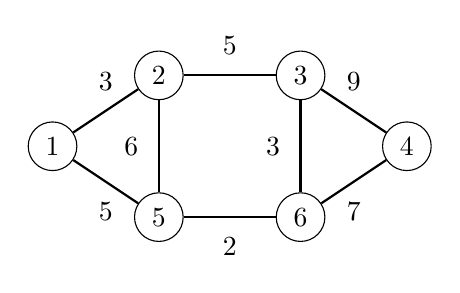
\begin{tikzpicture}[scale=0.9]
        \node[draw, circle] (1) at (1.5,2) {$1$};
        \node[draw, circle] (2) at (3,3) {$2$};
        \node[draw, circle] (3) at (5,3) {$3$};
        \node[draw, circle] (4) at (6.5,2) {$4$};
        \node[draw, circle] (5) at (3,1) {$5$};
        \node[draw, circle] (6) at (5,1) {$6$};
        \path[draw,thick,-] (1) -- node[font=\small,label=above:3] {} (2);
        \path[draw,thick,-] (2) -- node[font=\small,label=above:5] {} (3);
        \path[draw,thick,-] (3) -- node[font=\small,label=above:9] {} (4);
        \path[draw,thick,-] (1) -- node[font=\small,label=below:5] {} (5);
        \path[draw,thick,-] (5) -- node[font=\small,label=below:2] {} (6);
        \path[draw,thick,-] (6) -- node[font=\small,label=below:7] {} (4);
        \path[draw,thick,-] (2) -- node[font=\small,label=left:6] {} (5);
        \path[draw,thick,-] (3) -- node[font=\small,label=left:3] {} (6);
    \end{tikzpicture}
\end{center}

\pagebreak
El primer paso del algoritmo es ordenar las aristas por orden
creciente de sus pesos. El resultado es la siguiente lista:

\begin{center}
    \begin{tabular}{ll}
        \\
        nodo & peso \\
        \hline
        5--6 & 2    \\
        1--2 & 3    \\
        3--6 & 3    \\
        1--5 & 5    \\
        2--3 & 5    \\
        2--5 & 6    \\
        4--6 & 7    \\
        3--4 & 9    \\
        \\
    \end{tabular}
\end{center}

Luego de esto, el algoritmo recorre la lista y añade cada arista
al árbol si une dos componentes separados.

Inicialmente, cada nodo está en su propio componente:
\begin{center}
    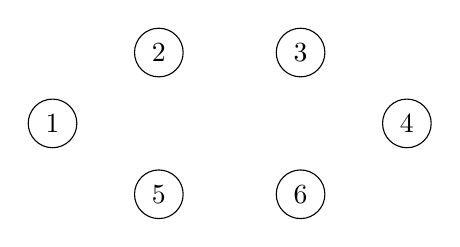
\begin{tikzpicture}[scale=0.9]
        \node[draw, circle] (1) at (1.5,2) {$1$};
        \node[draw, circle] (2) at (3,3) {$2$};
        \node[draw, circle] (3) at (5,3) {$3$};
        \node[draw, circle] (4) at (6.5,2) {$4$};
        \node[draw, circle] (5) at (3,1) {$5$};
        \node[draw, circle] (6) at (5,1) {$6$};
        %\path[draw,thick,-] (1) -- node[font=\small,label=above:3] {} (2);
        %\path[draw,thick,-] (2) -- node[font=\small,label=above:5] {} (3);
        %\path[draw,thick,-] (3) -- node[font=\small,label=above:9] {} (4);
        %\path[draw,thick,-] (1) -- node[font=\small,label=below:5] {} (5);
        %\path[draw,thick,-] (5) -- node[font=\small,label=below:2] {} (6);
        %\path[draw,thick,-] (6) -- node[font=\small,label=below:7] {} (4);
        %\path[draw,thick,-] (2) -- node[font=\small,label=left:6] {} (5);
        %\path[draw,thick,-] (3) -- node[font=\small,label=left:3] {} (6);
    \end{tikzpicture}
\end{center}

La primera arista a añadirse al árbol es la arista 5--6, que crea el
componente $\{5,6\}$ uniendo los componentes $\{5\}$ y $\{6\}$:

\begin{center}
    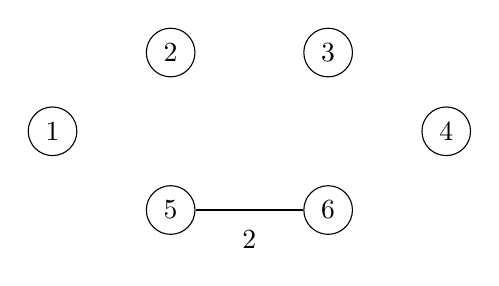
\begin{tikzpicture}
        \node[draw, circle] (1) at (1.5,2) {$1$};
        \node[draw, circle] (2) at (3,3) {$2$};
        \node[draw, circle] (3) at (5,3) {$3$};
        \node[draw, circle] (4) at (6.5,2) {$4$};
        \node[draw, circle] (5) at (3,1) {$5$};
        \node[draw, circle] (6) at (5,1) {$6$};

        %\path[draw,thick,-] (1) -- node[font=\small,label=above:3] {} (2);
        %\path[draw,thick,-] (2) -- node[font=\small,label=above:5] {} (3);
        %\path[draw,thick,-] (3) -- node[font=\small,label=above:9] {} (4);
        %\path[draw,thick,-] (1) -- node[font=\small,label=below:5] {} (5);
        \path[draw,thick,-] (5) -- node[font=\small,label=below:2] {} (6);
        %\path[draw,thick,-] (6) -- node[font=\small,label=below:7] {} (4);
        %\path[draw,thick,-] (2) -- node[font=\small,label=left:6] {} (5);
        %\path[draw,thick,-] (3) -- node[font=\small,label=left:3] {} (6);
    \end{tikzpicture}
\end{center}

Luego de esto, las aristas 1--2, 3--6, y 1--5 son añadidas similarmente:
\begin{center}
    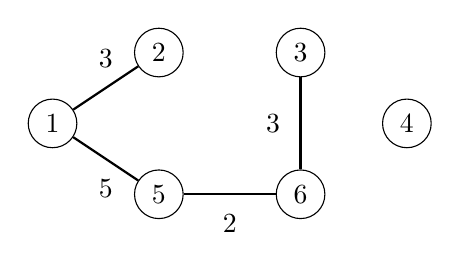
\begin{tikzpicture}[scale=0.9]
        \node[draw, circle] (1) at (1.5,2) {$1$};
        \node[draw, circle] (2) at (3,3) {$2$};
        \node[draw, circle] (3) at (5,3) {$3$};
        \node[draw, circle] (4) at (6.5,2) {$4$};
        \node[draw, circle] (5) at (3,1) {$5$};
        \node[draw, circle] (6) at (5,1) {$6$};

        \path[draw,thick,-] (1) -- node[font=\small,label=above:3] {} (2);
        %\path[draw,thick,-] (2) -- node[font=\small,label=above:5] {} (3);
        %\path[draw,thick,-] (3) -- node[font=\small,label=above:9] {} (4);
        \path[draw,thick,-] (1) -- node[font=\small,label=below:5] {} (5);
        \path[draw,thick,-] (5) -- node[font=\small,label=below:2] {} (6);
        %\path[draw,thick,-] (6) -- node[font=\small,label=below:7] {} (4);
        %\path[draw,thick,-] (2) -- node[font=\small,label=left:6] {} (5);
        \path[draw,thick,-] (3) -- node[font=\small,label=left:3] {} (6);
    \end{tikzpicture}
\end{center}

Después de estos pasos, la mayoría de los componentes se han unido y quedan
dos componentes en el árbol: $\{1,2,3,5,6\}$ y $\{4\}$.

La próxima arista en la lista es la 2--3, pero no será incluida
en el árbol porque los nodos 2 y 3 ya están en el mismo componente.
Por la misma razón la arista 2--5 no será incluida.

\begin{samepage}
    Finalmente, la arista 4--6 se añade al árbol:
    \begin{center}
        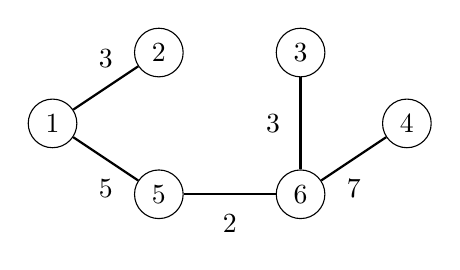
\begin{tikzpicture}[scale=0.9]
            \node[draw, circle] (1) at (1.5,2) {$1$};
            \node[draw, circle] (2) at (3,3) {$2$};
            \node[draw, circle] (3) at (5,3) {$3$};
            \node[draw, circle] (4) at (6.5,2) {$4$};
            \node[draw, circle] (5) at (3,1) {$5$};
            \node[draw, circle] (6) at (5,1) {$6$};

            \path[draw,thick,-] (1) -- node[font=\small,label=above:3] {} (2);
            %\path[draw,thick,-] (2) -- node[font=\small,label=above:5] {} (3);
            %\path[draw,thick,-] (3) -- node[font=\small,label=above:9] {} (4);
            \path[draw,thick,-] (1) -- node[font=\small,label=below:5] {} (5);
            \path[draw,thick,-] (5) -- node[font=\small,label=below:2] {} (6);
            \path[draw,thick,-] (6) -- node[font=\small,label=below:7] {} (4);
            %\path[draw,thick,-] (2) -- node[font=\small,label=left:6] {} (5);
            \path[draw,thick,-] (3) -- node[font=\small,label=left:3] {} (6);
        \end{tikzpicture}
    \end{center}
\end{samepage}

Luego de esto, el algoritmo deja de incluir aristas nuevas
porque el grafo está conexo y hay un camino entre cada par de
nodos. El grafo resultante es un árbol de expansión mínimo con peso
$2+3+3+5+7=20$.

\subsubsection{¿Por qué funciona?}

Es una buena pregunta por qué funciona este algoritmo. ¿Por qué
una estrategia voraz garantiza que encontraremos el árbol de expansión
mínimo?

Veamos qué sucede si la arista de peso mínimo del grafo \emph{no} es
incluida en el árbol. Por ejemplo, supongamos que un árbol de expansión
para el grafo previo no incluyera la arista de peso mínimo 5--6.
No sabemos la estructura exacta de tal árbol, pero en cualquier caso
debe contener algunas aristas. Asumamos que el árbol se vea así:
\begin{center}
    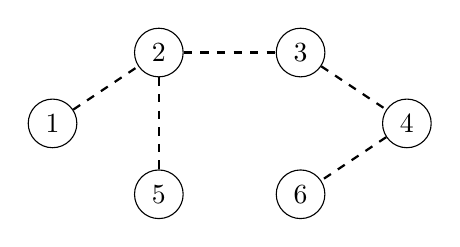
\begin{tikzpicture}[scale=0.9]
        \node[draw, circle] (1) at (1.5,2) {$1$};
        \node[draw, circle] (2) at (3,3) {$2$};
        \node[draw, circle] (3) at (5,3) {$3$};
        \node[draw, circle] (4) at (6.5,2) {$4$};
        \node[draw, circle] (5) at (3,1) {$5$};
        \node[draw, circle] (6) at (5,1) {$6$};

        \path[draw,thick,-,dashed] (1) -- (2);
        \path[draw,thick,-,dashed] (2) -- (5);
        \path[draw,thick,-,dashed] (2) -- (3);
        \path[draw,thick,-,dashed] (3) -- (4);
        \path[draw,thick,-,dashed] (4) -- (6);
    \end{tikzpicture}
\end{center}

No obstante, es imposible que este árbol sea un árbol mínimo para
el grafo, ya que podemos remover una arista del árbol y
reemplazarla con la arista mínima 5--6. Esto produce un árbol
de expansión cuyo peso es \emph{menor}:

\begin{center}
    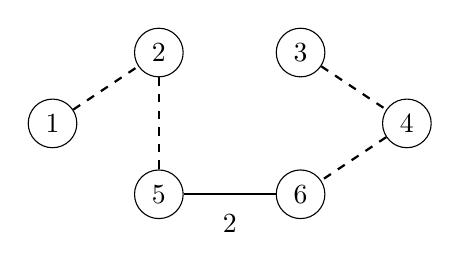
\begin{tikzpicture}[scale=0.9]
        \node[draw, circle] (1) at (1.5,2) {$1$};
        \node[draw, circle] (2) at (3,3) {$2$};
        \node[draw, circle] (3) at (5,3) {$3$};
        \node[draw, circle] (4) at (6.5,2) {$4$};
        \node[draw, circle] (5) at (3,1) {$5$};
        \node[draw, circle] (6) at (5,1) {$6$};

        \path[draw,thick,-,dashed] (1) -- (2);
        \path[draw,thick,-,dashed] (2) -- (5);
        \path[draw,thick,-,dashed] (3) -- (4);
        \path[draw,thick,-,dashed] (4) -- (6);
        \path[draw,thick,-] (5) -- node[font=\small,label=below:2] {} (6);
    \end{tikzpicture}
\end{center}

Por esta razón, siempre es óptimo incluir la arista de peso mínimo
en el árbol para producir un árbol de expansión mínimo. Utilizando
un argumento similar, podemos demostrar que también es óptimo añadir
la siguiente arista en orden por peso, y así sucesivamente.
Por lo tanto, el algoritmo de Kruskal funciona correctamente y
siempre produce un árbol de expansión mínimo.

\subsubsection{Implementación}

Implementando el algoritmo de Kruskal es conveniente representar
el grafo como una lista de aristas. La primera fase del algoritmo
ordena las aristas en $O(m \log m)$, y la segunda fase construye el
árbol de la siguiente manera:
\begin{lstlisting}
for (...) {
    if (!juntos(a, b)) unir(a,b);
}
\end{lstlisting}

El bucle recorre las aristas en la lista y siempre procesa una
arista $a$--$b$ donde $a$ y $b$ son dos nodos. Dos funciones son
necesarias: La función \texttt{juntos} determina si $a$ y $b$ están
en el mismo componente, y la función \texttt{unir} une los dos
componentes que contienen a $a$ y $b$.

El problema es cómo implementar eficientemente las funciones
\texttt{juntos} y \texttt{unir}. Una posibilidad es implementar
la función \texttt{juntos} como un recorrido de grafo y revisar si
podemos alcanzar el nodo $b$ desde el nodo $a$. No obstante, la
complejidad temporal de esta función sería $O(n+m)$ y el algoritmo
resultante sería muy lento, porque la función \texttt{juntos} será
llamada por cada nodo en el grafo.

Vamos a resolver este problema usando la estructura de unión--búsqueda
que implementa estas dos funciones en $O(\log n)$. Por ende, la
complejidad del algoritmo de Kruskal será de $O(m \log n)$ una vez
ordenadas las aristas.

\section{Estructura de unión--búsqueda}

\index{unión--búsqueda (estructura)}
\index{conjuntos disjuntos (estructura)}

La \key{estructura de unión--búsqueda}\footnote{También es conocida
    como \textit{estructura de conjuntos disjuntos} y
    por sus nombres en inglés \textit{disjoint set union} (DSU) y
    \textit{union-find} (UF-DS).} mantiene una colección de conjuntos
disjuntos, por lo que ningún elemento pertenece a más de un conjunto.
Soporta dos operaciones en $O(\log n)$: \texttt{unir} une dos
conjuntos en uno, y \texttt{buscar} encuentra el ``representante''
del conjunto que contenga al elemento dado.\footnote{La estructura
    presentada aquí fue introducida en 1971 por J. E. Hopcroft y
    J. D. Ullman \cite{hop71}. Luego, en 1975, R. E. Tarjan estudió
    una variante más sofisticada de la estructura \cite{tar75} que se
    describe en muchos libros de algoritmos hoy en día.}

\subsubsection{Estructura}

En esta estructura, un elemento en cada conjunto
es el \emph{representante} del conjunto, y hay una cadena de cualquier
otro elemento del conjunto a ese mismo. Por ejemplo, asume que tenemos
unos conjuntos $\{1,4,7\}$, $\{5\}$ y $\{2,3,6,8\}$:
\begin{center}
    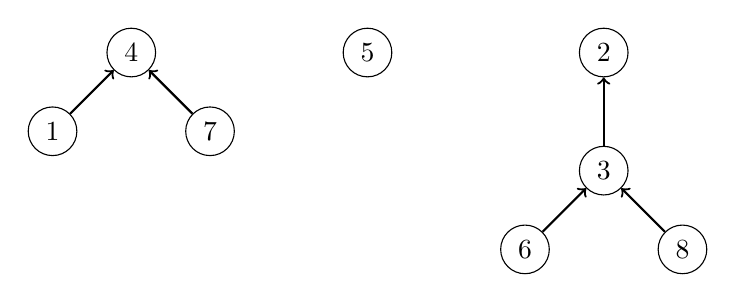
\begin{tikzpicture}
        \node[draw, circle] (1) at (0,-1) {$1$};
        \node[draw, circle] (2) at (7,0) {$2$};
        \node[draw, circle] (3) at (7,-1.5) {$3$};
        \node[draw, circle] (4) at (1,0) {$4$};
        \node[draw, circle] (5) at (4,0) {$5$};
        \node[draw, circle] (6) at (6,-2.5) {$6$};
        \node[draw, circle] (7) at (2,-1) {$7$};
        \node[draw, circle] (8) at (8,-2.5) {$8$};

        \path[draw,thick,->] (1) -- (4);
        \path[draw,thick,->] (7) -- (4);

        \path[draw,thick,->] (3) -- (2);
        \path[draw,thick,->] (6) -- (3);
        \path[draw,thick,->] (8) -- (3);

    \end{tikzpicture}
\end{center}

En este caso los representantes de cada conjunto son 4, 5, y 2.
Podemos encontrar el representante de cualquier elemento si seguimos
la cadena que comienza en ese elemento. Por ejemplo, el elemento 2 es
el representante del elemento 6, porque seguimos la cadena
$6 \rightarrow 3 \rightarrow 2$. Dos elementos pertenecen al mismo
conjunto si sus representantes son iguales.

Dos conjuntos pueden unirse si conectamos el representante
de un conjunto al representante del otro conjunto. Por ejemplo,
los conjuntos $\{1,4,7\}$ y $\{2,3,6,8\}$ se pueden unir de la
siguiente manera:
\begin{center}
    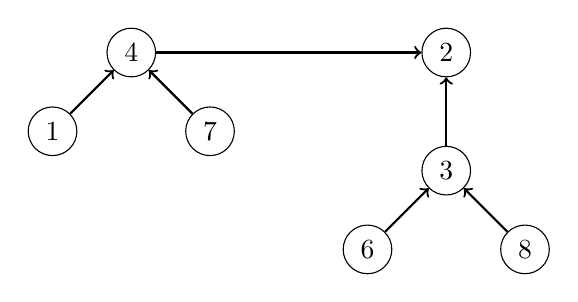
\begin{tikzpicture}
        \node[draw, circle] (1) at (2,-1) {$1$};
        \node[draw, circle] (2) at (7,0) {$2$};
        \node[draw, circle] (3) at (7,-1.5) {$3$};
        \node[draw, circle] (4) at (3,0) {$4$};
        \node[draw, circle] (6) at (6,-2.5) {$6$};
        \node[draw, circle] (7) at (4,-1) {$7$};
        \node[draw, circle] (8) at (8,-2.5) {$8$};

        \path[draw,thick,->] (1) -- (4);
        \path[draw,thick,->] (7) -- (4);

        \path[draw,thick,->] (3) -- (2);
        \path[draw,thick,->] (6) -- (3);
        \path[draw,thick,->] (8) -- (3);

        \path[draw,thick,->] (4) -- (2);
    \end{tikzpicture}
\end{center}

El conjunto resultante contiene los elementos $\{1,2,3,4,6,7,8\}$.
A partir de ahora, el elemento 2 es el representante del conjunto
entero, y el representante previo 4 apunta al elemento 2.

La eficiencia de la estructura de unión--búsqueda depende en cómo
se unan los conjuntos. Resulta que podemos seguir una simple estrategia:
siempre conectar el representante del conjunto \emph{más pequeño} al
representante del conjunto \emph{más grande}, si sus tamaños son distintos.
Usando esta estrategia, la longitud de cualquier cadena será $O(\log n)$,
por lo que podemos encontrar el representante de cualquier elemento
eficientemente si seguimos la cadena correspondiente.

\subsubsection{Implementación}

Podemos implementar la estructura de unión--búsqueda utilizando arreglos.
En la siguiente implementación, el arreglo \texttt{vecino} contiene, para
cada elemento, el siguiente elemento en la cadena o a sí mismo si el
elemento es un representante, y el arreglo \texttt{tamaño} indica, para
cada representante, el tamaño de su conjunto correspondiente.

Inicialmente, cada elemento pertenece a un conjunto diferente:
\begin{lstlisting}
for (int i = 1; i <= n; i++) vecino[i] = i;
for (int i = 1; i <= n; i++) tamaño[i] = 1;
\end{lstlisting}

La función \texttt{buscar} devuelve el representante para un elemento
$x$. El representante puede encontrarse si seguimos la cadena que
comienza en $x$.

\begin{lstlisting}
int buscar(int x) {
    while (x != vecino[x]) x = vecino[x];
    return x;
}
\end{lstlisting}

\newpage
La función \texttt{juntos} revisa si los elementos $a$ y $b$ pertenecen
al mismo conjunto. Esto es fácil utilizando la función \texttt{buscar}:

\begin{lstlisting}
bool juntos(int a, int b) {
    return buscar(a) == buscar(b);
}
\end{lstlisting}

La función \texttt{unir} une los dos conjuntos que contienen a los
elementos $a$ y $b$ (que deben pertenecer a diferentes conjuntos).
Primero encuentra el representante de cada conjunto
y luego conecta el más pequeño con el más grande.

\begin{lstlisting}
void unir(int a, int b) {
    a = buscar(a);
    b = buscar(b);
    if (tamaño[a] < tamaño[b]) swap(a, b);
    tamaño[a] += tamaño[b];
    vecino[b] = a;
}
\end{lstlisting}

La complejidad temporal de \texttt{buscar} es $O(\log n)$
asumiendo que la longitud de cada cadena es $O(\log n)$. En este caso,
\texttt{juntos} y \texttt{unir} también funcionan
en $O(\log n)$. La función \texttt{unir} se asegura de que la longitud
de cada cadena sea $O(\log n)$ cuando conecta conjuntos los conjuntos
más pequeños a los más grandes.

\section{Algoritmo de Prim}

\index{algoritmo de!Prim}

El \key{algoritmo de Prim}\footnote{El algoritmo lleva el nombre
    de R. C. Prim, quien lo publicó en 1957 \cite{pri57}. Sin
    embargo, el mismo algoritmo había sido descubierto en 1930
    por V. Jarnik.} es un método alternativo para construir
un árbol de expansión mínimo. Primero, el algoritmo añade un
nodo arbitrario al árbol. Luego, siempre elige una arista de
peso mínimo que añada un nuevo nodo al árbol. Finalmente, el árbol
está completo.

El algoritmo de Prim se asemeja al algoritmo de Dijkstra; la
diferencia es que el de Dijkstra siempre elige aristas
de distancia mínima, mientras que el algoritmo de Prim siempre
elige aristas de peso mínimo (que añadan un nodo).

\subsubsection{Ejemplo}

Veamos cómo funciona el algoritmo de Prim en el siguiente grafo:
\begin{center}
    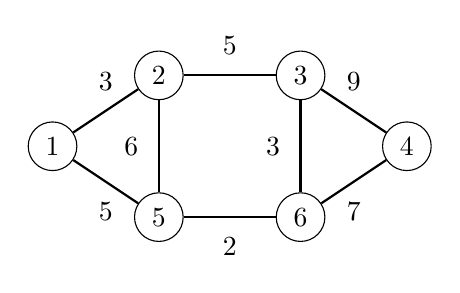
\begin{tikzpicture}[scale=0.9]
        \node[draw, circle] (1) at (1.5,2) {$1$};
        \node[draw, circle] (2) at (3,3) {$2$};
        \node[draw, circle] (3) at (5,3) {$3$};
        \node[draw, circle] (4) at (6.5,2) {$4$};
        \node[draw, circle] (5) at (3,1) {$5$};
        \node[draw, circle] (6) at (5,1) {$6$};
        \path[draw,thick,-] (1) -- node[font=\small,label=above:3] {} (2);
        \path[draw,thick,-] (2) -- node[font=\small,label=above:5] {} (3);
        \path[draw,thick,-] (3) -- node[font=\small,label=above:9] {} (4);
        \path[draw,thick,-] (1) -- node[font=\small,label=below:5] {} (5);
        \path[draw,thick,-] (5) -- node[font=\small,label=below:2] {} (6);
        \path[draw,thick,-] (6) -- node[font=\small,label=below:7] {} (4);
        \path[draw,thick,-] (2) -- node[font=\small,label=left:6] {} (5);
        \path[draw,thick,-] (3) -- node[font=\small,label=left:3] {} (6);

        %\path[draw=red,thick,-,line width=2pt] (5) -- (6);
    \end{tikzpicture}
\end{center}

Inicialmente, no hay ninguna arista entre los nodos:
\begin{center}
    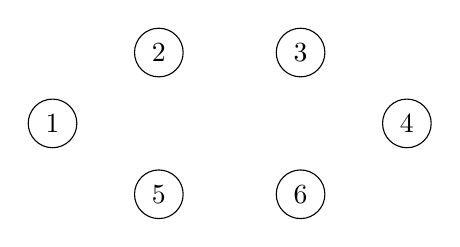
\begin{tikzpicture}[scale=0.9]
        \node[draw, circle] (1) at (1.5,2) {$1$};
        \node[draw, circle] (2) at (3,3) {$2$};
        \node[draw, circle] (3) at (5,3) {$3$};
        \node[draw, circle] (4) at (6.5,2) {$4$};
        \node[draw, circle] (5) at (3,1) {$5$};
        \node[draw, circle] (6) at (5,1) {$6$};
        %\path[draw,thick,-] (1) -- node[font=\small,label=above:3] {} (2);
        %\path[draw,thick,-] (2) -- node[font=\small,label=above:5] {} (3);
        %\path[draw,thick,-] (3) -- node[font=\small,label=above:9] {} (4);
        %\path[draw,thick,-] (1) -- node[font=\small,label=below:5] {} (5);
        %\path[draw,thick,-] (5) -- node[font=\small,label=below:2] {} (6);
        %\path[draw,thick,-] (6) -- node[font=\small,label=below:7] {} (4);
        %\path[draw,thick,-] (2) -- node[font=\small,label=left:6] {} (5);
        %\path[draw,thick,-] (3) -- node[font=\small,label=left:3] {} (6);
    \end{tikzpicture}
\end{center}

Un nodo arbitrario puede ser el nodo inicial, así que elegimos el nodo 1.
Primero, añadimos el nodo 2 que está conectado por una arista de peso 3:
\begin{center}
    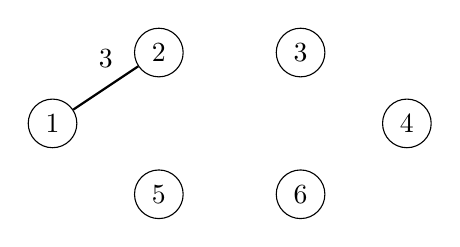
\begin{tikzpicture}[scale=0.9]
        \node[draw, circle] (1) at (1.5,2) {$1$};
        \node[draw, circle] (2) at (3,3) {$2$};
        \node[draw, circle] (3) at (5,3) {$3$};
        \node[draw, circle] (4) at (6.5,2) {$4$};
        \node[draw, circle] (5) at (3,1) {$5$};
        \node[draw, circle] (6) at (5,1) {$6$};
        \path[draw,thick,-] (1) -- node[font=\small,label=above:3] {} (2);
        %\path[draw,thick,-] (2) -- node[font=\small,label=above:5] {} (3);
        %\path[draw,thick,-] (3) -- node[font=\small,label=above:9] {} (4);
        %\path[draw,thick,-] (1) -- node[font=\small,label=below:5] {} (5);
        %\path[draw,thick,-] (5) -- node[font=\small,label=below:2] {} (6);
        %\path[draw,thick,-] (6) -- node[font=\small,label=below:7] {} (4);
        %\path[draw,thick,-] (2) -- node[font=\small,label=left:6] {} (5);
        %\path[draw,thick,-] (3) -- node[font=\small,label=left:3] {} (6);
    \end{tikzpicture}
\end{center}

Luego de esto, hay dos aristas con peso 5, así que podemos añadir
el nodo 3 o el nodo 5 al árbol. Probemos con 3 primero:
\begin{center}
    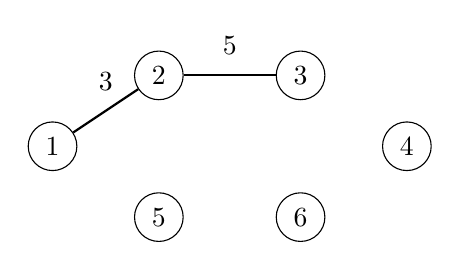
\begin{tikzpicture}[scale=0.9]
        \node[draw, circle] (1) at (1.5,2) {$1$};
        \node[draw, circle] (2) at (3,3) {$2$};
        \node[draw, circle] (3) at (5,3) {$3$};
        \node[draw, circle] (4) at (6.5,2) {$4$};
        \node[draw, circle] (5) at (3,1) {$5$};
        \node[draw, circle] (6) at (5,1) {$6$};
        \path[draw,thick,-] (1) -- node[font=\small,label=above:3] {} (2);
        \path[draw,thick,-] (2) -- node[font=\small,label=above:5] {} (3);
        %\path[draw,thick,-] (3) -- node[font=\small,label=above:9] {} (4);
        %\path[draw,thick,-] (1) -- node[font=\small,label=below:5] {} (5);
        %\path[draw,thick,-] (5) -- node[font=\small,label=below:2] {} (6);
        %\path[draw,thick,-] (6) -- node[font=\small,label=below:7] {} (4);
        %\path[draw,thick,-] (2) -- node[font=\small,label=left:6] {} (5);
        %\path[draw,thick,-] (3) -- node[font=\small,label=left:3] {} (6);
    \end{tikzpicture}
\end{center}

El proceso continúa hasta que todos los nodos formen parte del árbol:
\begin{center}
    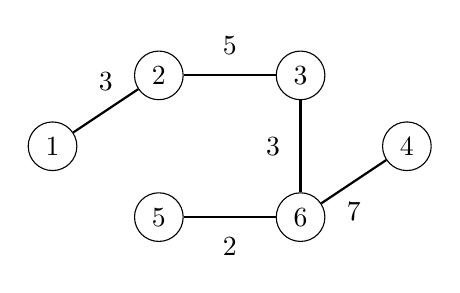
\begin{tikzpicture}[scale=0.9]
        \node[draw, circle] (1) at (1.5,2) {$1$};
        \node[draw, circle] (2) at (3,3) {$2$};
        \node[draw, circle] (3) at (5,3) {$3$};
        \node[draw, circle] (4) at (6.5,2) {$4$};
        \node[draw, circle] (5) at (3,1) {$5$};
        \node[draw, circle] (6) at (5,1) {$6$};
        \path[draw,thick,-] (1) -- node[font=\small,label=above:3] {} (2);
        \path[draw,thick,-] (2) -- node[font=\small,label=above:5] {} (3);
        %\path[draw,thick,-] (3) -- node[font=\small,label=above:9] {} (4);
        %\path[draw,thick,-] (1) -- node[font=\small,label=below:5] {} (5);
        \path[draw,thick,-] (5) -- node[font=\small,label=below:2] {} (6);
        \path[draw,thick,-] (6) -- node[font=\small,label=below:7] {} (4);
        %\path[draw,thick,-] (2) -- node[font=\small,label=left:6] {} (5);
        \path[draw,thick,-] (3) -- node[font=\small,label=left:3] {} (6);
    \end{tikzpicture}
\end{center}

\subsubsection{Implementación}

Tal como el algoritmo de Dijkstra, el algoritmo de Prim se puede
implementar eficientemente utilizando una cola de prioridad. La
cola de prioridad debería contener todos los nodos que pueden
ser conectados al componente actual utilizando una sola arista,
en orden creciente de los pesos de las aristas correspondientes.

La complejidad temporal del algoritmo de Prim es
$O(n + m \log m)$, igual a aquella del algoritmo de Dijkstra.
En la práctica, los dos algoritmos de Prim y de Kruskal son eficientes,
y la elección es una cuestión de gusto. No obstante, la mayoría de
programadores competitivos eligen el algoritmo de Kruskal.